

\tikzset{every picture/.style={line width=0.75pt}} %set default line width to 0.75pt        

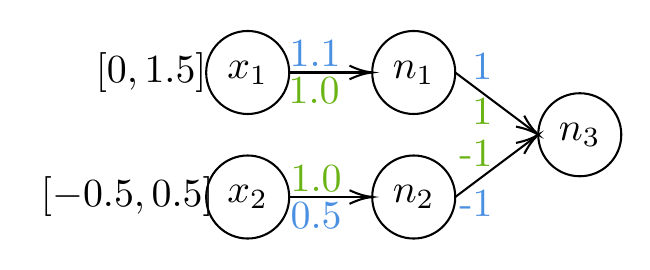
\begin{tikzpicture}[x=0.75pt,y=0.75pt,yscale=-1,xscale=1]
%uncomment if require: \path (0,300); %set diagram left start at 0, and has height of 300

%Shape: Circle [id:dp06612404457840415] 
\draw   (80,60) .. controls (80,48.95) and (88.95,40) .. (100,40) .. controls (111.05,40) and (120,48.95) .. (120,60) .. controls (120,71.05) and (111.05,80) .. (100,80) .. controls (88.95,80) and (80,71.05) .. (80,60) -- cycle ;
%Shape: Circle [id:dp685015234974003] 
\draw   (80,120) .. controls (80,108.95) and (88.95,100) .. (100,100) .. controls (111.05,100) and (120,108.95) .. (120,120) .. controls (120,131.05) and (111.05,140) .. (100,140) .. controls (88.95,140) and (80,131.05) .. (80,120) -- cycle ;
%Shape: Circle [id:dp36531807362590973] 
\draw   (160,60) .. controls (160,48.95) and (168.95,40) .. (180,40) .. controls (191.05,40) and (200,48.95) .. (200,60) .. controls (200,71.05) and (191.05,80) .. (180,80) .. controls (168.95,80) and (160,71.05) .. (160,60) -- cycle ;
%Shape: Circle [id:dp8605838523620923] 
\draw   (160,120) .. controls (160,108.95) and (168.95,100) .. (180,100) .. controls (191.05,100) and (200,108.95) .. (200,120) .. controls (200,131.05) and (191.05,140) .. (180,140) .. controls (168.95,140) and (160,131.05) .. (160,120) -- cycle ;
%Shape: Circle [id:dp18951934248445623] 
\draw   (240,90) .. controls (240,78.95) and (248.95,70) .. (260,70) .. controls (271.05,70) and (280,78.95) .. (280,90) .. controls (280,101.05) and (271.05,110) .. (260,110) .. controls (248.95,110) and (240,101.05) .. (240,90) -- cycle ;
%Straight Lines [id:da2027373665168457] 
\draw    (120,60) -- (158,60) ;
\draw [shift={(160,60)}, rotate = 180] [color={rgb, 255:red, 0; green, 0; blue, 0 }  ][line width=0.75]    (10.93,-3.29) .. controls (6.95,-1.4) and (3.31,-0.3) .. (0,0) .. controls (3.31,0.3) and (6.95,1.4) .. (10.93,3.29)   ;

%Straight Lines [id:da534577266557194] 
\draw    (120,120) -- (158,120) ;
\draw [shift={(160,120)}, rotate = 180] [color={rgb, 255:red, 0; green, 0; blue, 0 }  ][line width=0.75]    (10.93,-3.29) .. controls (6.95,-1.4) and (3.31,-0.3) .. (0,0) .. controls (3.31,0.3) and (6.95,1.4) .. (10.93,3.29)   ;

%Straight Lines [id:da6712362717076668] 
\draw    (200,120) -- (238.4,91.2) ;
\draw [shift={(240,90)}, rotate = 503.13] [color={rgb, 255:red, 0; green, 0; blue, 0 }  ][line width=0.75]    (10.93,-3.29) .. controls (6.95,-1.4) and (3.31,-0.3) .. (0,0) .. controls (3.31,0.3) and (6.95,1.4) .. (10.93,3.29)   ;

%Straight Lines [id:da7166627548154052] 
\draw    (200,60) -- (238.4,88.8) ;
\draw [shift={(240,90)}, rotate = 216.87] [color={rgb, 255:red, 0; green, 0; blue, 0 }  ][line width=0.75]    (10.93,-3.29) .. controls (6.95,-1.4) and (3.31,-0.3) .. (0,0) .. controls (3.31,0.3) and (6.95,1.4) .. (10.93,3.29)   ;


% Text Node
\draw (132.5,51) node [scale=1.44,color={rgb, 255:red, 74; green, 144; blue, 226 }  ,opacity=1 ] [align=left] {1.1};
% Text Node
\draw (133,129) node [scale=1.44,color={rgb, 255:red, 74; green, 144; blue, 226 }  ,opacity=1 ] [align=left] {0.5};
% Text Node
\draw (213,57) node [scale=1.44,color={rgb, 255:red, 74; green, 144; blue, 226 }  ,opacity=1 ] [align=left] {1};
% Text Node
\draw (210,99) node [scale=1.44,color={rgb, 255:red, 105; green, 179; blue, 20 }  ,opacity=1 ] [align=left] {\mbox{-}1};
% Text Node
\draw (100,60) node [scale=1.44]  {$x_1$};
% Text Node
\draw (100,120) node [scale=1.44]  {$x_2$};
% Text Node
\draw (53.5,60) node [scale=1.44]  {$[ 0,1.5]$};
% Text Node
\draw (42,120) node [scale=1.44]  {$[ -0.5,0.5]$};
% Text Node
\draw (180,60) node [scale=1.44]  {$n_{1}$};
% Text Node
\draw (180,120) node [scale=1.44]  {$n_{2}$};
% Text Node
\draw (260,90) node [scale=1.44]  {$n_{3}$};
% Text Node
\draw (132,69) node [scale=1.44,color={rgb, 255:red, 105; green, 179; blue, 20 }  ,opacity=1 ] [align=left] {1.0};
% Text Node
\draw (133,111) node [scale=1.44,color={rgb, 255:red, 105; green, 179; blue, 20 }  ,opacity=1 ] [align=left] {1.0};
% Text Node
\draw (213,79) node [scale=1.44,color={rgb, 255:red, 105; green, 179; blue, 20 }  ,opacity=1 ] [align=left] {1};
% Text Node
\draw (210,123) node [scale=1.44,color={rgb, 255:red, 74; green, 144; blue, 226 }  ,opacity=1 ] [align=left] {\mbox{-}1};


\end{tikzpicture}

